\documentclass[12pt]{article}
\usepackage{geometry}
\geometry{a4paper}
\usepackage[round]{natbib}
\usepackage{graphicx}
\usepackage[T1]{fontenc}
\usepackage[utf8]{inputenc}
\usepackage{textcomp}
\usepackage{gensymb}
\usepackage{hyperref}
\usepackage{amsmath}
\usepackage{amssymb}
\usepackage{authblk}
\usepackage[running]{lineno}
\usepackage{setspace}
\usepackage{rotating}

\setlength{\parindent}{0pt}


\usepackage{fancyhdr}
 
\pagestyle{fancy}
\fancyhf{}
\rhead{Tad Dallas (Biol 4253)}
\lhead{ Host-parasite interactions}

\doublespacing


\begin{document}




\subsection*{Reading:}

Kilpatrick, A. M. \& Altizer, S. (2010) Disease Ecology. Nature Education Knowledge 3(10):55 \\ \url{https://www.nature.com/scitable/knowledge/library/disease-ecology-15947677}










\begin{center}
\noindent\hrulefill 
\end{center}



\clearpage






\subsection*{What are the effects of parasites?}

Host-parasite interactions are a type of consumer-resource interaction, where the resource is the host, and the consumer is the parasite. Here, the interaction is characterized by a gain for the parasite and a loss for the host, fundamentally differing from other symbioses such as mutualism or competition. \\


Parasites are a diverse group. Pretty much every group of living thing has a parasite, including parasites (a parasite of a parasite is called a \textit{hyperparasite}). The diversity of life history strategies, transmission modes, and lifestyles make parasites unique. Parasites infect a set of hosts, referred as the \textit{host range} or the set of \textit{permissive hosts}. Meanwhile, hosts harbor any number of parasite species, which is referred as that hosts \textit{parasite species richness}. Parasites may be \textit{specialists} (infecting only a single host species) or quite \textit{generalists} (infecting a broad range of host species). \\


Apart from the impacts of parasites on human health, agricultural crops, and livestock, parasites provide an interesting system to study and test fundamental ecological theory (some of which we've touched on previously). For instance, we can apply concepts from population dynamics to model the effect of parasites on host population dynamics. Previously, scientists demonstrated that infection of red grouse by a parasitic nematode caused the grouse population to exhibit cycles. 












\subsection*{What are the types of parasites?}

There are a quite a few ways to divide parasites into functional groups. \\

First, the location on the host can determine parasite grouping with \textit{endoparasites} being inside the host (e.g., cestode) and \textit{ectoparasites} living on the outside of the host (e.g., tick). \\

Second, the size of the parasite itself can be a grouping (though this is slightly subjective), with \textit{microparasites} typically referring to those parasites that are too small to see with the naked eye and that reproduce within the host, and \textit{macroparasites}, which are larger and reproduce outside of the host. Examples of microparasites would be fungal parasites, bacteria, viruses. Examples of macroparasites would be helminths, arthropods like ticks and fleas. A confusing one would be botflies, which are large dipteran parasites which deposit a single larvae under the skin of the host, which emerges as an adult. \\ 


Third, parasite transmission mode can be horizontal (from organism to organism), vertical (from mother to offspring), or environmental (through the environment). \\













\bigskip
\subsection*{The parasite niche}

The parasite niche is defined in a similar manner as the niche of a free-living species. That is, abiotic tolerances are important in describing the parasite niche. However, parasite lifecycle controls to what extent environmental axes are true niche axes. For instance, a parasite species which is only ever exposed to the internal environment of the host should not have a niche axis related to the temperature of the external environment, as this is unlikely to directly influence parasite persistence. For this parasite, in particular, the environment \textit{is} the host individual, such that an appropriate niche axis might relate more to some property of the host. The characterization of the parasite niche is important to understanding the geographic distribution of a parasite. That is, we can imagine situations where the environment is ideal for a parasite, but there are no \textit{permissive} host species present, so the parasite cannot persist. We can also imagine a situation where a permissive host species is present, but the environment too harsh and the parasite cannot persist in these conditions. \\



Apart from using the niche concept to understand a parasite species geographic distribution, the niche concept also can allow for the estimation of \textit{host switching} potential. That is, what is the probability that a parasite can infect any given novel host, when it has not previously been found to infect this host. Host switching is important, as it can lead to \textit{spillover} events, if the host switching involves the ability to infect a human host. There may be a set of host traits which allow the prediction of host switching. That is, hosts that are more similar to known hosts of a parasite might be more likely to become infected. This makes sense in light of niche concepts, as host phylogenetic distance may represent a niche axis, along which more closely related hosts would be more likely to become infected. However, not all niche concepts can be mapped onto parasites as easy. For instance, defining persistence for a parasite which may have epidemic-like dynamics is difficult (though not impossible, as we'll discuss in the R0 section). \\











\bigskip

\subsection*{Parasite life cycle complexity}

Many parasites do not simply complete their life cycle on one or more host species directly (e.g., a mosquito may feed on a subset of species directly), but instead require multiple species to complete a single generation. For instance, each segment of a tapeworm is a reproductive entity containing "eggs". These eggs are found in the feces of infected hosts. Cows which graze in these areas may consume trematodes, and larval trematodes can encyst within the muscle tissue of the host. Then humans eat the cows and get infected. This is a simple example. A more complex, and perhaps better example, is that of another trematode parasite, which has four life stages -- egg, cercariae, metacercariae, and adult -- all of which infect different host species. 




\begin{figure}
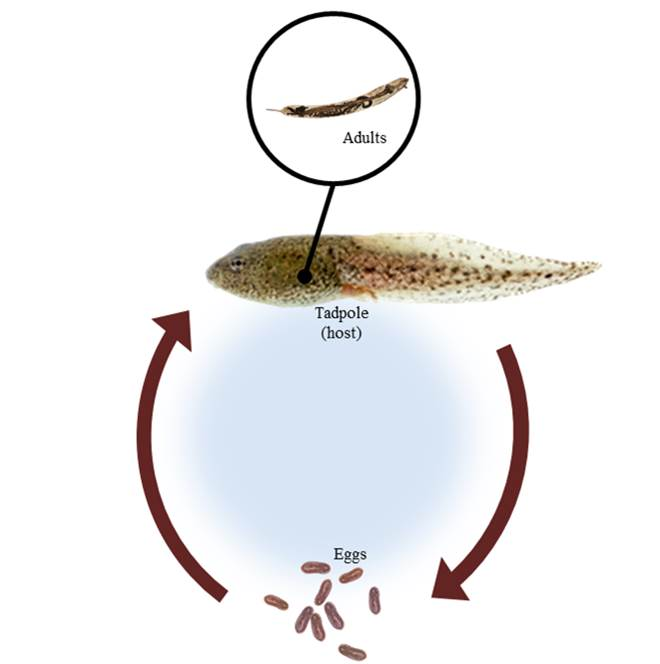
\includegraphics[width=0.75\textwidth]{figs/DirectLifeCycle.jpg}
\caption{Example of a direct (or simple) life cycle parasite.}
\end{figure}


\begin{figure}
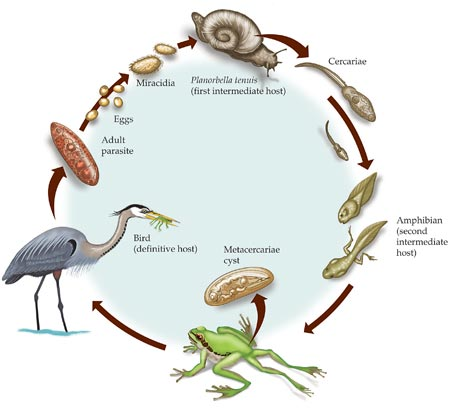
\includegraphics[width=0.75\textwidth]{figs/IndirectLifeCycle.jpg}
\caption{Example of a complex life cycle parasite.}
\end{figure}

















\bigskip
\subsection*{Modeling host-parasite interactions}

Despite the variety of parasite life history and transmission modes, one flexible model which can capture many fundamental aspects of host-parasite infection dynamics is the SIR model. This is a compartmental model where host individuals can be either susceptible (S), infected (I), or recovered/removed (R). Other forms of this simple model exist, including latent periods after transmission but before the host becomes infectious (E for exposed), as well as extensions for multi-host scenarios, recovery with waning immunity (i.e., recovered individuals get susceptible at some rate), and others. \\


\begin{align}
\frac{dS}{dt} &=  -\beta SI\\
\frac{dI}{dt} &=  \beta SI - dI \\
\frac{dR}{dt} &=  dI
\end{align}


where $\beta$ is the transmission rate and $d$ is parasite-induced mortality or the recovery rate, depending if the $R$ class are dead or recovered with immunity. $1/d$ is the average infectious period. Importantly, we are modeling the proportions of a fixed-size population, such that $S+I+R = N$. More specifically, we often only care about the relative proportion of each class, and assume some scaling. That is, $\frac{S}{N}+\frac{I}{N}+\frac{R}{N} = 1$.





\paragraph*{Model Assumptions:}
\begin{itemize}
	\item Mass Action
	\item Same susceptibility for every individual
	\item All outbreaks of same disease alike
\end{itemize}














% Made it to about here last time

Here, the basic reproductive number ($R_0$) describes the number of secondary infections generated by a single infected individual in a wholly susceptible population. 


\begin{equation}
R_0 = \frac{\beta}{d}
\end{equation}



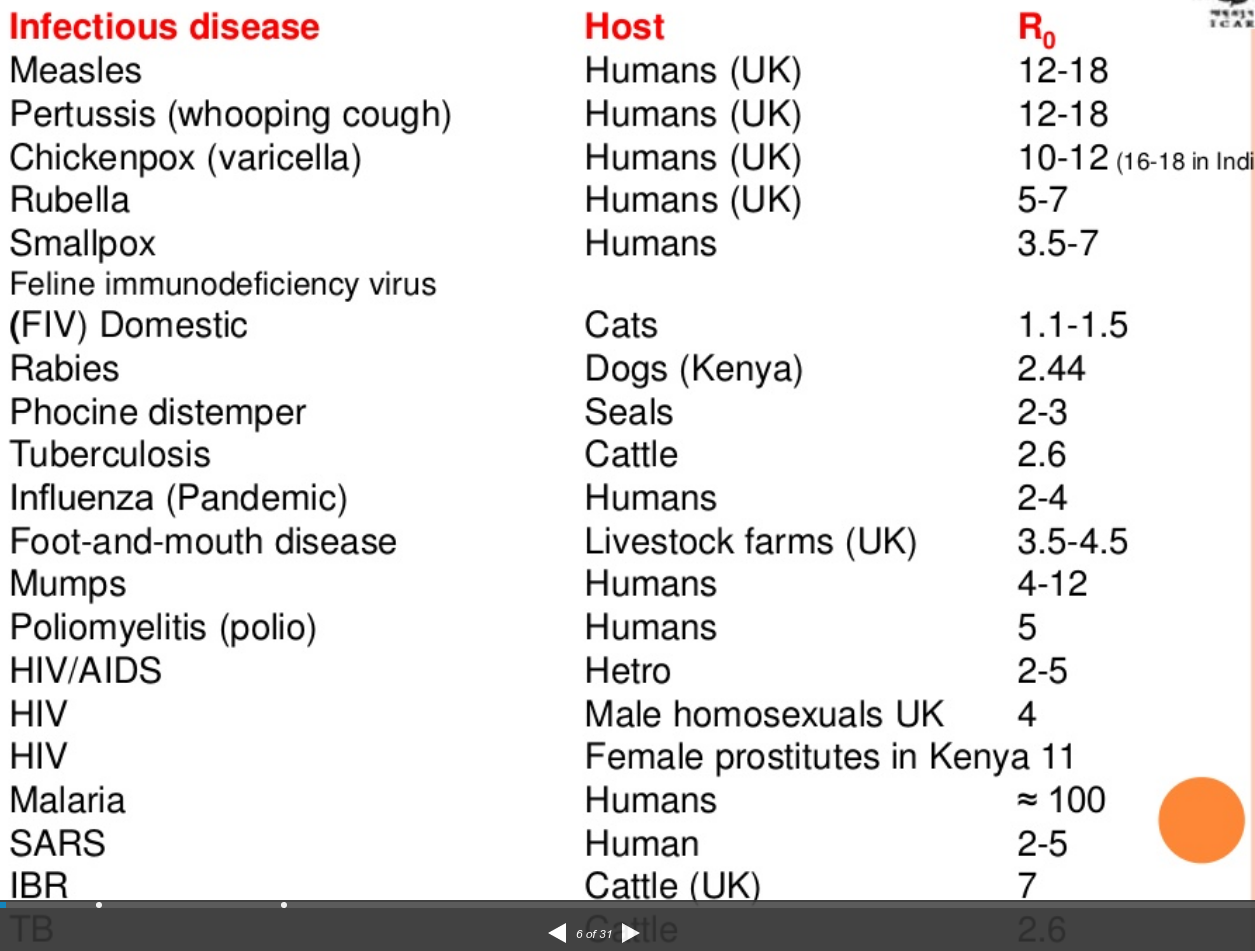
\includegraphics[width=0.75\textwidth]{figs/r0.png}




One useful thing about estimating $R_0$ is that it essentially allows the estimation of the probability that a pathogen will invade a given host population (called a \textit{pathogen invasion threshold}). That is, $R_0 >=$ 1 causes pathogen invasion, while $R_0 <$ 1 means the pathogen does not invade. Also, we can look at each component of $R_0$, and get an idea of how to control a disease. That is, $R_0$ is made up of two terms:


\begin{itemize}
  \item $\beta$ the transmission rate
  \item $d$ parasite-induced mortality (\textit{or} recovery rate)
\end{itemize}


If $d$ is big, the pathogen cannot invade. If $\beta$ is small, the pathogen cannot invade. \\


Loosely speaking, the outcome of an initial pathogen infection event in the SIR model can have 3 possible outcomes. First, the $R_0$ is below 1, and the infected individual moves to the recovered/removed class without causing any further infection. Second, the pathogen invades, infects a bunch of people, and then leaves the population (an epidemic pathogen). Third, the pathogen invades, and maintains sustained low levels of infection in the population (an endemic pathogen). \\


Another related quantity to $R_0$ is the \textit{force of infection}, which is simply $\beta I$, which captures the transmission rate times the number of infected individuals (a measure which is proportional to transmission potential to the susceptible population $S$.














\paragraph*{How do we reduce $R_0$?}

The model above is simple, in that it assumes direct transmission (infected individuals transmit pathogen as soon as they are infected at the same rate until they recover or die). What other things could influence $R_0$? \\


What if the pathogen is vector-borne (i.e., transmitted by a mosquito or other insect)? \\

What if the pathogen has a latent period after transmission before the host becomes infectious? \\

\textit{Can you think of other things that would influence $R_0$}? 














\paragraph*{Vaccination}

One way we could reduce pathogen invasion is through vaccination. What happens if we can pre-emptively treat some fraction of the population? It is possible to vaccinate enough of the population that the $R_0$ is reduced below 1, and the entire population is not susceptible to pathogen invasion. This is called \textit{herd immunity}, and the threshold fraction of the population required to vaccinate to achieve herd immunity is $1 - \frac{1}{R_0}$. This is because, $R_0$ is the number of secondary cases given a wholly susceptible population $S$. If we can reduce $S$, we can actually reduce the risk that any one single infection will propagate.  











\subsubsection*{A couple of examples demonstrating why simple models may miss key things}

The classic SIR model makes a whole bunch of assumptions. 

\paragraph*{Superspreaders} 

One of which is that individuals are equally good at becoming infected, and have an equal number of contacts. This may not be true though. For instance, during the spread of Typhoid fever in the early 1900's, Mary Mallon was an asymptomatic carrier of Typhoid, \textit{and} worked in a job where she had many more contacts than the average person (a cook). She infected over 50 people with Typhoid. 



\paragraph*{A well-mixed population}

All individuals are modeled to interact with all other individuals, such that we don't need to worry about the variation in contact rates or spatial structure. In London, there was a cholera outbreak in 1854. Cholera is transmitted through contaminated water, which wasn't really known at the time (they thought cholera was caused by "bad air"). John Snow was a physician who mapped out cases of cholera, and found that most of the cases were spatially aggregated around one water pump (Broad Street Pump). He applied enough pressure to the city council to have this pump handle removed, albeit temporarily, which may have caused the epidemic to decline. 

















\bigskip

\subsection*{Evolution of virulence and the Red Queen}

But $R_0$ isn't necessarily a static quantity, but can potentially change through time. This occurs for a number of reasons. One of the reasons is that transmission parameters can change. \\



Virulence ($d$ in the SIR model) should evolve to be relatively low, as parasites need their hosts, right? However, parasites that replicate too slowly may not pass on their genes to future generations, and damage to the host is inevitable for many parasite species. This leads to questions about how virulence should change over time for a given parasite, which has lead to a large body of research on virulence evolution.   \\



Hosts and parasites are in a constant arms race, where hosts evolve resistance mechanisms to the pathogen, and the pathogen evolves ways to get around these host defenses. This process of host-parasite co-evolution is referred to as \textit{Red Queen} dynamics. \\





\textit{A good example:}\\

A mixed sexual and asexual (clonal) population of snails was exposed to a pathogen. They found that over time, the asexual (clonal) types disappeared entirely due to infection pressure, while the sexual types were able to develop a resistance to the pathogen. This is evidence for one aspect of the Red Queen (the parasite drives host evolution). \\


The other aspect is the evolution of the parasite to overcome host defenses. We've documented this often, in terms of virus evolution to evade detection from the host immune system, among other examples. \\









































\clearpage


\subsection*{Environmental controls of disease spread}

The environment influences infection dynamics in a number of ways.  \\

First, the environment could influence the transmission process. An example of this would be if host individuals encountered a pathogen at higher rates in warmer environments. This would happen if foraging behavior of the host increased, pathogen shedding rate increased (the rate at which the pathogen is dispersed from an infected individual), or environmental pathogen survival increased at higher temperatures. This gets back to niche concepts, as marginally higher temperatures might increase transmission, but very high temperatures will reduce transmission, and potentially kill host and/or pathogen. A good example of this is \textit{Daphnia} species that are infected with a yeast pathogen can be cleared of pathogen ("cured" in a sense) after exposure to UV light. The UV kills the pathogen, but the host can tolerate it (to a certain point).  \\


Second, the environment could influence the growth of pathogen within an infected host. To keep the same environmental factor, elevated temperature can cause increased pathogen growth rates inside infected host individuals, which could result in increased virulence or increased pathogen load (number of infectious units per infected host individual). Elevated temperature could also stress host immune function, leading to a reduced ability of the host to fight off infection. Recall that elevated temperature could also simulate a "fever response", where immune function is enhanced at warmer temperatures. \\



Third, the environment can control host or vector behavior. For instance, host individuals exposed to rising temperatures might seek refuge (use habitat differently) which could enhance parasite transmission. More frequent drought can shift host distributions in space and may enhance or reduce parasite transmission. In terms of the vector behavior, a good example is when there is an interaction between infection status of a vector and the environment. Mosquitoes infected by Plasmodium (the pathogen which causes malaria) tend to prefer to occupy warmer habitats, which increases pathogen growth. That is, the pathogen modifies the host behavior to enhance the growth of the pathogen within the host individual. \\











\bigskip

\subsection*{Land use change and disease spread}

Human land use change has influenced pathogen spillover events (when zoonotic pathogens infecting wildlife transfer to human populations). There are a number of reasons for this, partly related to the environmental effects discussed above, and partly to due with how land use change influences host communities. \\

For starters, land use change results in increased contact of wildlife and human populations, which can potentially enable zoonotic pathogens to spillover into human populations. \\


Land use change also alters host communities, as some species are less affected by disturbance. These species tend to become more abundant in disturbed landscapes, and are often pretty competent disease carriers. Here, competence means that the host individual is good at carrying and spreading the pathogen. An example would be that white-footed mice are found in higher abundance in urban and disturbed environments. These mice are also really competent vectors of a number of diseases (e.g. Lyme disease). An example not related only to vector-borne disease is the spread of a horizontally transmitted pathogen of house sparrows (conjunctivitis) in urban environments. Food supplementation (bird feeders, etc.) has caused these birds to come in close contact with other bird species (and with other individuals of their own species). This close contact has lead to the infection prevalence (percent of individuals infected) being higher in urban environments (where contact rates between birds are higher) than in more natural environments. 


















\bigskip
\subsection*{Community composition and disease spread}

Host species differ in their susceptibility (ability to become infected) and suitability (ability to transmit parasites). On top of this, most parasite species infect more than one host species. Therefore, the diversity of host species present in a given site may influence the resulting parasite infection dynamics. These relationships are often referred to as \textit{diversity-disease} relationships. On one hand, increased host diversity may reduce overall parasite burden or abundance through the addition of host species which are less suitable, lowering overall transmission risk or parasite abundance. This is called a \textit{dilution effect}. On the other hand, if species in more diverse communities are \textbf{more} suitable, this would likely increase overall transmission risk or parasite abundance, leading to an \textit{amplification effect}. \\



Evidence for the dilution effect comes from a Lyme disease system, where the white-footed mouse is a competent host for Lyme disease, and is also super common. The presence of other, less competent, hosts reduces encounters of ticks with the most competent host (the white-footed mouse). \\



However, this requires that there is a direct relationship between host abundance and host competence, which is not really always the case (it rarely is).\\








\bigskip

\subsection*{Social contact networks and disease invasion/spread}

The SIR model which we introduced assumes a well-mixed population, which doesn't really incorporate spatial structure or variation in contact rates among individuals. Let's sketch out how networks are typically structured and how they might influence pathogen spread. 


\begin{itemize}
  \item Number of links
  \item Clustering of interactions
  \item Directionality of links (e.g., river networks)
  \item Variation in transmission (as a function of distance between individuals, etc.)
\end{itemize}













\textbf{Why are social contact networks essential in some situations?} \\

Sexual contact networks are often really variable in terms of number of links per person, and considering the structure of the network is super important to understanding the spread of sexually-transmitted infections. \\

Designing vaccination strategies should incorporate information on the structure of the network (larger bodied individuals tend to have more links, etc.) \\


Fragmenting the network into groups is a good way at isolating and protecting subgroups of nodes (e.g., will draw an example of this in the notes). The idea is that we can fragment the network into two subgroups that aren't connected, even if the pathogen invades one part of the network, the other will be great. \\






































\end{document}
